\chapter{C++ 使用与双语言对比试验}
\label{chap:dual-language}

\section{语言分工与安装}

完整 MATLAB 包位于 \code{matlab/}，包含原有求解器、模型、公共接口、图形、MAT 文件保存与读取、全部正式和历史示例。原生 C++17 包位于 \code{cpp/}，不依赖 MATLAB、MATLAB Runtime 或 MEX；顶层 \code{CMakeLists.txt} 只构建 C++。本说明书、论文草稿、投稿元数据和 \code{experiments/} 为两种语言共享。MATLAB 从仓库根目录执行 \code{addpath('matlab/tools')} 后调用 \code{setup_ddpack}；外部旧脚本中的安装路径需要相应更新。

C++ 需要 CMake 3.20 以上、C++17 编译器与 Eigen 3.4 以上。先在系统中安装 Eigen，或者配置时用 \code{-DDDPACK_EIGEN_DIR=/path/to/eigen} 指定其源码目录。Linux/macOS 的典型命令如下；Windows 使用 Visual Studio 时在配置命令中追加 \code{-G "Visual Studio 17 2022" -A x64}，可执行文件位于 \code{build/Release/}。
\begin{lstlisting}[language=bash]
cmake -S . -B build -DCMAKE_BUILD_TYPE=Release
cmake --build build --config Release --parallel 2
ctest --test-dir build -C Release --output-on-failure
./build/ddpack_examples all artifacts/native_run_001
./build/ddpack_examples obstacle_3d artifacts/native_3d_001
\end{lstlisting}
每次选择新的输出目录。结果包含 \code{states.csv}、\code{controls.csv}、\code{time.csv}、代价历史、\code{metrics.json}、\code{config.json} 与环境记录。C++ 不生成 MATLAB 的 figure 或 MAT 文件。

\section{C++ 接口和扩展范围}

公共头文件为 \code{cpp/include/ddpack/ddpack.hpp}，安装后的 CMake 链接目标为 \code{DDPACK::ddpack}。\code{Problem} 保存初始状态、目标状态、动力学、代价、控制界和物理验收条件；\code{Options} 选择算法与迭代参数；\code{Solution} 保存轨迹、物理时间、目标、迭代历史和独立诊断。二维数组采用 Eigen 矩阵，状态和控制的每一列对应一个时间节点。最后一个控制列仅为接口补齐，动力学和代价使用前 $N-1$ 列。

以下代码示意接口；完整的九个配置见 \code{cpp/examples/problems.cpp}，独立安装消费示例见 \code{cpp/tests/consumer/}。
\begin{lstlisting}[language=C++]
#include <ddpack/ddpack.hpp>
ddpack::Problem p;
// Set x0, target, u_max, tf, dt, dynamics and cost.
ddpack::Options options;
options.algorithm = ddpack::Algorithm::free_time_pddp;
auto solution = ddpack::solve(p, options);
if (!solution.metrics.success) { /* inspect diagnostics */ }
ddpack::write_artifacts(p, options, solution, "new_result");
\end{lstlisting}

六个维护算法的 ID 与 MATLAB 一致。原生扩展要求自主连续动力学 $f(x,u)$、运行代价密度、终端代价及一致的解析导数；内置线性/仿射模型、摆、平面模型、三维飞行模型和热过程。标量约束采用 $G(x,u)\ge0$ 可行约定，目前只在自由时间 PDDP 和惩罚型自由时间 DDP 分支启用。制导种子仍按固定 0.1 s 步长生成控制；终端缺陷及几何分支再限幅并按实际求解网格积分初始状态。相应模型维数限制仍适用，不能由接口形式推断其支持任意状态维数、非自主模型或任意约束。

独立模型检查接口另位于 \code{<ddpack/derivatives.hpp>}：
\code{check_derivatives(p,x,u)} 返回局部导数与函数值检查记录。安装消费示例同时编译并调用该接口。
它不需要 MATLAB，也不在优化器热路径中自动执行；原生回调保持自主物理时间约定。

\section{对比设计与复现入口}

试验 A 检查相同问题设置下的数值与物理结果；试验 B 测量完整公共求解接口的耗时。九个案例覆盖六种维护算法。两种实现使用相同的状态初值、目标、代价权重、网格、控制界、参数、迭代上限、投影设置与物理阈值，不启用 QuickMode。\code{comparison_case} 直接读取正式 MATLAB 示例的配置段，\code{parameters.json} 保存权重和参数；分析脚本核对原生输出中的算法、网格和迭代参数。振动案例使用 MATLAB \code{rng(4)} 生成的同一组初始控制，C++ 读取已冻结的 CSV；每次 MATLAB 求解前恢复随机状态。

两种语言分别预热 3 次，再测量 5 次；依次运行，不同时运行两个求解程序。计时包括公共求解入口的校验、优化与诊断；MATLAB 使用 \code{evalc} 捕获求解器输出，该开销在计时内。配置构造、随机状态恢复、绘图、文件写入、程序启动及 C++ 编译均不计时。报告中位数与按线性插值定义的第 25/75 百分位数，不作显著性检验。本机为 Windows 11、Intel Core i5-12500H；MATLAB 为 R2023b（记录计算线程数为 1），C++ 为 MSVC 19.44 Release x64、Eigen 5.0.0。没有强制两套实现使用相同线程数。

在仓库根目录运行 MATLAB：
\begin{lstlisting}
addpath('matlab/tools');
setup_ddpack('IncludeBenchmarks',true);
run_language_comparison(fullfile(pwd,'artifacts','my_comparison','matlab'));
\end{lstlisting}
MATLAB 结束后运行 C++ 和 Python 汇总（Python 需要 NumPy 与 Matplotlib）：
\begin{lstlisting}[language=bash]
./build/ddpack_benchmark cpp/tests/reference artifacts/my_comparison/cpp
python experiments/analyze.py --matlab artifacts/my_comparison/matlab --cpp artifacts/my_comparison/cpp --output experiments/results
\end{lstlisting}
完整原始计时、配置、物理指标、误差和输入文件哈希见 \code{experiments/results/}；完整轨迹和求解日志写入指定的 \code{artifacts/} 子目录。冻结 MATLAB 轨迹另随 \code{cpp/tests/reference/} 分发。表与图由分析脚本从实测数据生成，重新测量会产生不同的耗时。

\section{误差定义与结果}

轨迹误差定义为
\[
 \Delta x_\infty=\max_{i,k}|x^M_{i,k}-x^C_{i,k}|,\qquad
 \Delta u_\infty=\max_{j,k<N}|u^M_{j,k}-u^C_{j,k}|.
\]
归一化误差以 MATLAB 参考数组绝对最大值与 1 的较大者为分母。混合量纲的绝对分量差只用于实现回归，物理验收仍使用各案例自己的终端误差、控制界、净空及动力学缺陷阈值。物理时间轴逐节点比较；本次九例最终时间差在数值舍入范围内。

为避免求解历史记录与最终返回轨迹的语义差异，两种轨迹的目标统一由同一个分析函数重新计算：
\[
 J=\tfrac12(x_N-x_f)^\top Q_f(x_N-x_f)
  +\sum_{k=1}^{N-1}\Delta t_k
   \left[\tfrac12(x_k-x_f)^\top Q_s(x_k-x_f)
   +\tfrac12u_k^\top Ru_k+c\right],
\]
其中惩罚型自由时间 DDP 的 $c=1$，其余案例为 0。2026-11-13 修复后，终端缺陷返回目标与独立重算一致，历史记录中的代价滞后差异已移除。偏差仍单独输出以供审计，表中 $|\Delta J|$ 使用统一重算值。本节九例性能和轨迹数据均已在修复后顺序重跑。

\begin{table}[H]\centering\small
\caption{同输入完整求解对比：耗时中位数及四分位区间，单位 ms；每例每语言 5 次。}
\begin{tabular}{lrrr}\toprule
案例 & MATLAB & C++ & 中位数比值\\\midrule
Vibration & 47.63 [47.32, 51.59] & 5.65 [5.25, 6.28] & 8.43\\
Planar & 61.29 [57.98, 62.20] & 6.74 [6.63, 6.97] & 9.09\\
Terminal defect & 50.84 [50.27, 56.05] & 5.91 [5.89, 5.99] & 8.60\\
Obstacle 2D & 612.02 [608.07, 631.89] & 23.69 [23.40, 23.71] & 25.84\\
Obstacle 3D & 412.12 [404.77, 423.34] & 80.08 [79.04, 81.05] & 5.15\\
Reactor & 11.50 [11.08, 12.00] & 1.60 [1.59, 1.60] & 7.20\\
Pendulum & 1260.07 [1259.01, 1267.34] & 129.09 [126.52, 130.12] & 9.76\\
Thermal & 183.91 [183.13, 185.65] & 21.55 [21.24, 21.71] & 8.53\\
Storage & 68.05 [67.80, 71.01] & 10.40 [10.03, 10.71] & 6.54\\
\bottomrule\end{tabular}\end{table}
\begin{table}[H]\centering\small
\caption{双语言的轨迹误差与物理终端误差。$\Delta x_\infty$、$\Delta u_\infty$ 为绝对分量最大差。}
\begin{tabular}{lrrrr}\toprule
案例 & $\Delta x_\infty$ & $\Delta u_\infty$ & 终端误差 M & 终端误差 C++\\\midrule
Vibration & 3.11e-15 & 4.66e-15 & 2.19e-03 & 2.19e-03\\
Planar & 5.11e-15 & 5.55e-15 & 1.22e-04 & 1.22e-04\\
Terminal defect & 5.33e-15 & 2.00e-15 & 3.15e-07 & 3.15e-07\\
Obstacle 2D & 4.80e-14 & 2.09e-13 & 1.75e-06 & 1.75e-06\\
Obstacle 3D & 2.61e-13 & 8.50e-13 & 7.88e-06 & 7.88e-06\\
Reactor & 4.88e-15 & 5.00e-16 & 3.14e-02 & 3.14e-02\\
Pendulum & 5.77e-15 & 5.33e-15 & 2.15e-06 & 2.15e-06\\
Thermal & 2.66e-15 & 0.00e+00 & 9.17e-08 & 9.17e-08\\
Storage & 5.00e-16 & 0.00e+00 & 3.22e-06 & 3.22e-06\\
\bottomrule\end{tabular}\end{table}
\begin{table}[H]\centering\small
\caption{独立四子步 RK4 缺陷、返回目标差与几何净空。无障碍案例以 -- 标记不适用。}
\begin{tabular}{lrrrrr}\toprule
案例 & RK4 M & RK4 C++ & $|\Delta J|$ & 净空 M & 净空 C++\\\midrule
Vibration & 5.91e-02 & 5.91e-02 & 8.88e-16 & -- & --\\
Planar & 1.78e-15 & 1.78e-15 & 3.55e-15 & -- & --\\
Terminal defect & 1.78e-15 & 1.78e-15 & 0.00e+00 & -- & --\\
Obstacle 2D & 1.66e-03 & 1.66e-03 & 3.55e-15 & 4.99e-03 & 4.99e-03\\
Obstacle 3D & 9.81e-04 & 9.81e-04 & 5.77e-15 & 5.00e-03 & 5.00e-03\\
Reactor & 1.57e-02 & 1.57e-02 & 3.55e-14 & -- & --\\
Pendulum & 3.37e-02 & 3.37e-02 & 8.88e-16 & -- & --\\
Thermal & 1.84e-02 & 1.84e-02 & 3.55e-15 & -- & --\\
Storage & 3.30e-05 & 3.30e-05 & 1.78e-15 & -- & --\\
\bottomrule\end{tabular}\end{table}

\begin{figure}[H]
\centering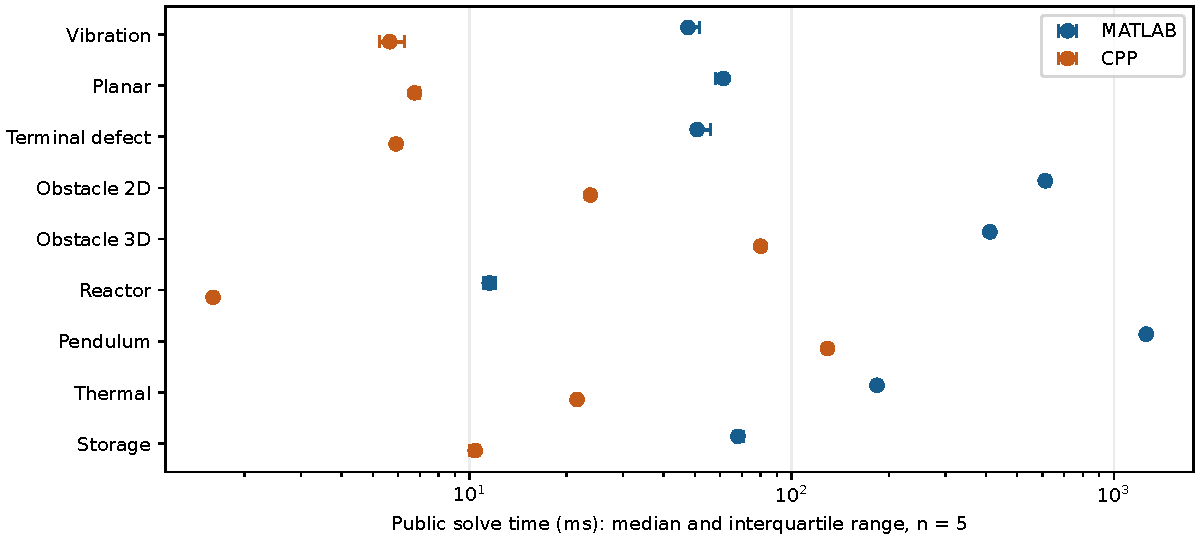
\includegraphics[width=\textwidth]{generated/timing.pdf}
\caption{本机完整接口耗时。点为中位数，横线为四分位区间；横轴为对数坐标。}
\end{figure}
\begin{figure}[H]
\centering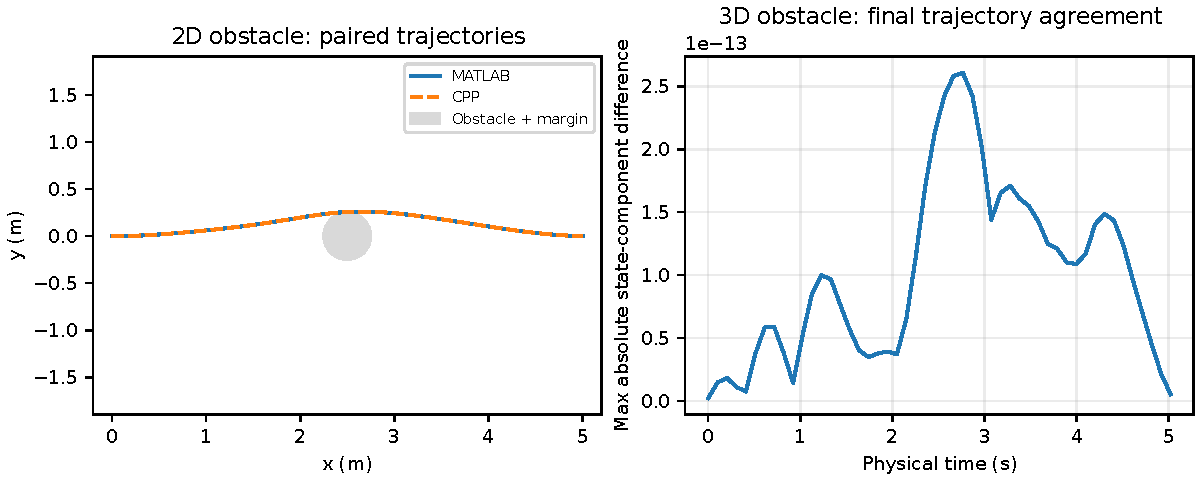
\includegraphics[width=\textwidth]{generated/trajectory_agreement.pdf}
\caption{左：二维避障轨迹重合；灰色区域为障碍物与物理安全裕度。右：三维案例各节点的最大绝对状态分量差，核对重启阶段输出的一致性。}
\end{figure}

九例的两种语言均通过各自的物理验收；Euler 一致性缺陷为浮点舍入量级。独立 RK4 缺陷并不等于零，它反映当前 Euler 网格相对于更高精度积分的误差，不能由较小的跨语言差异替代。九例完整轨迹高度一致；新二维、三维避障的最大状态分量差分别约 $4.80\times10^{-14}$ 和 $2.61\times10^{-13}$，活动控制差约 $2.09\times10^{-13}$ 和 $8.50\times10^{-13}$。两例均通过原终端误差、控制界、精确线段净空与独立积分检查。

CTest 对所有九例最终状态和活动控制使用统一的 $2\times10^{-6}$ 归一化阈值，不再对三维最终轨迹放宽容差。主迭代首轮检查 $10^{-9}$ 误差；终端缺陷及几何分支的全部实际 merit 试探记录和历史另以 $10^{-8}$ 检查。确定性重启阶段的候选记录和下降历史使用 $10^{-8}$，最终返回目标使用 $10^{-9}$。这些是当前九例的回归契约，不是任意问题的逐步等价证明。

\section{结果解释}
运行时间比值描述记录机器上完整实现的综合差异；五次重复与单台机器不能证明普遍性能优势。
MATLAB 与原生 C++ 的接口范围以本章和头文件为准。局部离散检查不等于全程连续模型验证。

\subsection{解析回放的双语言验收}
MATLAB 与 C++ 均对支持的恒速几何模型检查解析零阶保持回放。
结果字段分别为 \code{analytic_zoh_clearance_lower_bound} 和
\code{analytic_zoh_terminal_error}；前者必须非负，后者必须满足终端容差。
二者是独立于 Euler 节点的模型验证，不是算法全局最优性证明。
正式轨迹主图只展示当前解，双语言表继续比较相同输入下的 MATLAB 与 C++。
